\chapter{Implementación} \label{ich:implementacion}

Las nuevas técnicas que introducimos implican un esfuerzo considerable en la implementación de módulos de código. Como comentamos en \customref{isubsubs:observaciones_conclusiones_pksampling}, el uso de \textit{P-K sampling} provoca que no podamos usar librerías de aprendizaje automático para realizar tareas comunes, como muestreo de datos, funciones de pérdida, métricas, \ldots

Por tanto, en esta sección explicaremos todo el trabajo de implementación realizado.

\section{Control de versiones y buenas prácticas} \label{isec:github_buenas_practicas}

Para el control de versiones, usamos \textit{Git} con \textit{Github}. Todo el desarrollo del trabajo, tanto la implementación de código como la escritura de la presente memoria, se ha realizado en un repositorio abierto alojado en \cite{informatica:repogithub}.

Gracias al uso de \textit{Github} hemos podido implementar fácilmente una serie de buenas prácticas de desarrollo, entre las cuales se encuentran:

\begin{itemize}
    \item El uso de \textbf{\textit{issues}} para especificar las necesidades del proyecto en cada momento, los errores encontrados durante el proceso de implementación, \ldots. Véase por ejemplo \url{https://github.com/SergioQuijanoRey/TFG/issues/14}, donde especificamos una necesidad y proponemos una solución. Además, se pueden ver todos los \textit{commits} que tratan con dicha \textit{issue}
    \item Gracias a estar usando \textit{issues}, trabajamos con la metodología de \textbf{\textit{feature branches}}. En esta metodología, por cada nueva característica a implementar, se crea una \textit{branch} de \textit{Git} para introducir los cambios. Una vez se implementa y valida dicha característica, el código de la nueva \textit{branch} se fusiona en la rama principal \cite{informatica:feature_branches}. Como se puede ver en \cite{informatica:repogithub}, el nombre de cada \textit{feature branch} referencia al identificador de la \textit{issue} con la que estamos trabajando
    \item El fusionado de \textit{feature branches} a la rama principal se realiza por medio de \textbf{\textit{pull requests}}. En cada \textit{pull request} podemos revisar el código una última vez antes de fusionarlo en la rama principal. Además, sirven como forma de localizar los cambios de alto nivel introducidos en nuestra base de código. En nuestro caso, los \textit{commits} individuales pueden llegar a ser demasiado granulares, y revisando la lista de todos los \textit{commits} realizados podemos perder el foco sobre la tarea de alto nivel que tratan de resolver. Por ejemplo, en una \textit{pull request} como \url{https://github.com/SergioQuijanoRey/TFG/pull/57} podemos ver que, para introducir las dos variantes de \textit{Rank@K accuracy} (véase \customref{isubs:rank_at_k}) empleamos 53 \textit{commits}.
    \item El uso de \textbf{\textit{Github Actions}} para ejecutar ciertas tareas tras realizar una subida de \textit{commits} al repositorio (\entrecomillado{push}) o antes de aceptar una \textit{pull request}. Principalmente, hemos usado estas \entrecomillado{actions} para lanzar todos los \textit{tests} unitarios tras cada \textit{push} al repositorio y lanzar todos los \textit{tests} de integración antes de cada \textit{pull request}. El objetivo de esta base de \textit{tests} se especifica en \customref{isec:test_suite}
    \item El uso de \textbf{\textit{Github Projects}}, que nos ofrecen una tabla tipo \entrecomillado{Kanban} para organizar las tareas pendientes. Dicha forma de organizarnos ha sido ya comentada en \customref{isec:planificacion}.
\end{itemize}

\section{Entorno de ejecución}

Durante la implementación del código y el proceso de experimentación, hemos trabajado en tres entornos de desarrollo y ejecución distintos:

\begin{enumerate}
    \item El entorno de \textbf{desarrollo local}, nuestro ordenador portátil. Lo hemos usado principalmente para implementar el código y ejecutar algunos \textit{tests}. Por su baja potencia, no lo hemos usado ni para lanzar los \textit{Notebooks} de \textit{Jupyter} sobre los que realizamos la exploración de datos, ni para lanzar los \textit{scripts} de aprendizaje. Por tanto, no resulta interesante mostrar sus especificaciones

    \item En fases tempranas del proyecto hemos escrito y ejecutado código en \textbf{\textit{Google Colab}}. Esta plataforma nos permite ejecutar, a través de una interfaz \textit{web}, \textit{Notebooks} de \lstinline{Python}.

        \begin{itemize}
            \item Además, otorga de forma limitada algunos recursos como acceso a cómputo \textit{TPU}. Las \textit{Tensor Processing Units} o \textit{TPUs} son tecnología \textit{hardware} propietaria de \textit{Google}, que busca optimizar el entrenamiento e inferencia de modelos de IA \cite{informatica:google_tpu}.

            \item Los \textit{Notebooks} vienen con la mayoría de bibliotecas de aprendizaje automático pre-instaladas. Esto es una gran ventaja al inicio del desarrollo, puesto que evitamos enfrentarnos a la complejidad de configurar un entorno de ejecución \lstinline{Python} con las librerías necesarias

            \item Sin embargo, rápidamente tenemos que abandonar este entorno por dos motivos: el acceso a recursos es demasiado limitado, y solo poder usar código escrito en \textit{Notebooks} es una restricción importante.

            \item El \textit{hardware} que se pone a disposición del usuario se asigna dinámicamente, en base al consumo previo de recursos del usuario y a la demanda actual. Por tanto, no podemos obtener una especificación estática de los recursos de los que disponemos \cite{informatica:google_colab_faq}. Tampoco existe documentación oficial donde se especifique qué \textit{hardware} se ofrece, cuotas de consumo, \ldots\; Sin embargo, accediendo a un \textit{Notebook}, podemos ejecutar algunos comandos para ver los recursos que nos ofrecen en un momento dado \footnote{Dichos comandos son ejecutados el 18 de Septiembre de 2023}

                \begin{itemize}
                    \item El comando \lstinline{df -h} nos muestra que tenemos disponibles 50GB de memoria permanente. Sin embargo, esto no es una limitación porque podemos conectar nuestra cuenta de usuario de \textit{Google} para acceder a todos los datos almacenados en \textit{Google Drive}
                    \item El comando \lstinline{cat /proc/cpuinfo} nos muestra que estamos usando una \textit{CPU} \entrecomillado{Intel ( R ) Xeon ( R ) @ 2.20 GHz}
                    \item El comando \lstinline{cat /proc/meminfo} nos muestra que disponemos de aproximadamente 12GB de memoria \textit{RAM}
                    \item Sabemos que podemos acceder a \textit{TPUs} de \textit{Google}, pero no disponemos de ningún comando para acceder a las especificaciones de esta
                \end{itemize}
        \end{itemize}

    \item Los \textbf{clúster de servidores GPU de la Universidad de Granada, \textit{nGPU}}.
        \begin{itemize}
            \item Estos servidores se encuentran en el Centro de Procesado de Datos (\textit{CPD}) Santa Lucía. Para trabajar con estos servidores, accedemos por \lstinline{ssh} a un nodo cabecera, y usando el programa \lstinline{slurm}, enviamos trabajos a los distintos nodos que componen el \textit{CPD}.
            \item Hemos usado estos servidores tanto para lanzar \textit{Notebooks} en los que realizamos principalmente análisis exploratorio de datos, como para lanzar \textit{scripts} de \lstinline{Python} usados principalmente para llevar a cabo el entrenamiento y validación de modelos
            \item Los nodos \textit{Titan} y \textit{Atenea}, los dos nodos que hemos usado mayoritariamente, disponen del siguiente \textit{hardware}:
                \begin{itemize}
                    \item Dos \textit{Intel® Xeon® E5-2630}, cada uno
                    \item Memoria \textit{RAM} de 128 Gb \textit{DDR4}
                    \item Memoria permantente de 2,7TB
                    \item El nodo \textit{Titan} dispone de tres \textit{GPUs} \textit{GTX Titan X Pascal} y una \textit{GPU} \textit{GTX Titan Xp}, mientras que el nodo \textit{Atenea} dispone de cuatro \textit{GPUs} \textit{GTX Titan Xp}
                \end{itemize}
        \end{itemize}

\end{enumerate}
\todo{Esto debería ir a materiales}

Como lenguaje de programación usaremos \lstinline{Python}, en su versión 3.10.2. Para la gestión de entornos de \lstinline{Python} usaremos dos tecnologías:

\begin{enumerate}
    \item El gestor de paquetes y entornos \textbf{\lstinline{Conda}} \cite{informatica:conda_web}. Este gestor nos permite instalar fácilmente paquetes de \lstinline{Python} en entornos virtuales, evitando así instalarlos a nivel de sistema (lo que puede provocar conflictos con versiones de paquetes usados en otros proyectos). Además, permite generar un archivo \lstinline{enviroment.yml} que especifica exactamente qué paquetes están instalados y con qué versión. A partir de dicho fichero podremos reproducir el entorno de desarrollo en diferentes máquinas (por ejemplo, tenemos en mismo entorno de desarrollo en nuestro ordenador portátil y en los servidores donde se ejecutan los entrenamientos). Junto con el uso de contenedores \lstinline{docker} (enfoque que consideramos muy complejo), es la única alternativa que tenemos para configurar nuestro entorno de desarrollo en los servidores \textit{nGPU}
    \item \textbf{\lstinline{nix}} \cite{informatica:nixos_web}. Dicha tecnología se compone de un lenguaje funcional puro, que se usa en su gestor de paquetes reproducible y declarativo. Usamos esta tecnología en nuestro ordenador por su robustez: durante los meses de desarrollo, algunas librerías se rompen en sus últimas versiones. Con \lstinline{nix} podemos volver cómodamente a versiones previas de todo el entorno de desarollo (\entrecomillado{rollback}). Esto se puede conseguir también con \lstinline{Conda} pero es mucho más complicado. Además, permite especificar paquetes de \lstinline{Python}, paquetes de \LaTeX usados para producir esta memoria y paquetes de \textit{Linux}
\end{enumerate}

Como sistema operativo, hemos usado:

\begin{itemize}
    \item En nuestro entorno de desarrollo, la distribución de \textit{Linux} \textit{NixOS} en su versión 23.11
    \item En \textit{Google Colab}, la distribución de \textit{Linux} \textit{Ubuntu} en su versión 22.04.2 \textit{LTS} \footnote{Comprobamos esta versión ejecutando el comando \lstinline{lsb_release -d} el 19 de Septiembre de 2023}
    \item En los servidores \textit{nGPU}, la distribución de \textit{Linux} \textit{Ubuntu} en su versión 20.04.5 \textit{LTS}
\end{itemize}


\section{Estructura de carpetas del proyecto} \label{isec:estructura_carpetas}

Por la extensión de la base de código, es necesario que comentemos la estructura de carpetas del proyecto. En el directorio raíz tenemos los siguientes ficheros relevantes:

\begin{itemize}
    \item \lstinline{flake.nix} y \lstinline{flake.lock} especifican el entorno de desarrollo usando el gestor \textit{nix}. El fichero \lstinline{enviroment.yml} especifica el entorno de desarrollo usando el gestor \textit{Conda}
    \item Los ficheros \lstinline{interactive_slurm.sh} y \lstinline{launch_server_process.sh} son dos \textit{scripts Bash} que usamos para lanzar procesos en los servidores \textit{nGPU}. El primero lo utilizamos para entrar en una terminal de forma interactiva. El segundo, para lanzar un \textit{script} de \lstinline{Python} para que ejecute el aprendizaje y validación de un modelo
    \item \lstinline{justfile} especifica tareas para ejecutarse con la herramienta \lstinline{just} \cite{informatica:just}. Dicha herramienta es parecida a \lstinline{make}. La usamos para definir tareas como:
        \begin{itemize}
            \item Sincronizar las bases de código entre los tres entornos distintos con los que hemos trabajado
            \item Ejecutar ciertos \textit{scripts}
            \item Ejecutar la \textit{suite} de pruebas y los \textit{benchmarks}
            \item Ejecutar ciertos análisis estáticos sobre la base de código (usando \lstinline{mypy} y \lstinline{ruff})
            \item \ldots
        \end{itemize}
    \item \lstinline{optuna_queries.sql} define las consultas \lstinline{SQL} necesarias para vigilar el proceso de \textit{hyperparameter tuning}, que especificaremos en \customref{isec:hp_tuning}
\end{itemize}

En el directorio raíz del proyecto tenenos los siguientes subdirectorios:

\begin{itemize}
    \item \lstinline{.github/workflows} en el que definimos las \textit{Github Actions} que ejecutamos (véase \customref{isec:github_buenas_practicas})
    \item \lstinline{thesis} donde desarrollamos los documentos que componen la presente memoria
    \item \lstinline{src} donde realizamos todo el desarrollo de código. Este a su vez se divide en los siguientes subdirectorios:
        \begin{itemize}
            \item \lstinline{lib}, donde implementamos toda la librería que usamos en los \textit{Notebooks} y en los \textit{scripts} de entrenamiento. Implementan tareas varias, como el cálculo de funciones de pérdida, el \textit{P-K sampling}, métricas, bucles de entrenamiento, el sistema de \textit{logging}, \ldots
            \item \lstinline{test} e \lstinline{integration_tests} donde alojamos toda la \textit{suite} de pruebas unitarias y de integración, para validar las implementaciones realizadas en nuestra librería
            \item \lstinline{benchmarks} donde alojamos los \textit{benchmarks} empleados en \customref{isec:optimizacion_codigo}
            \item \lstinline{profiling} contiene los datos generados en los \textit{benchmarks} y el proceso explicado de optimización basado en datos
        \end{itemize}
    \item En \lstinline{src} tenemos algunos ficheros relevantes:

        \begin{itemize}
            \item \textit{Jupyter Notebooks} donde realizamos análisis exploratorios de distintas bases de datos
            \item \textit{Scripts} de \lstinline{Python}, usados principalmente para entrenar y validar modelos
        \end{itemize}\end{itemize}

\section{Estructura lógica de la base de código} \label{isec:estructura_paquetes_modulos}

En \customref{isec:estructura_carpetas} ya hemos hablado de la estructura de carpetas de la base de código. Ahora pasamos a comentar la estructura lógica de la base de código. Nos centraremos en la parte de la librería, pues en los \textit{Notebooks} y \textit{scripts} de \lstinline{Python} consumimos la librería para realizar análisis exploratorio de datos, entrenamiento de modelos y validación (véase \customref{isec:pipeline}).

Empezamos mostrando el diagrama de paquetes de nuestra librería:

\begin{figure}[H]
    \centering
    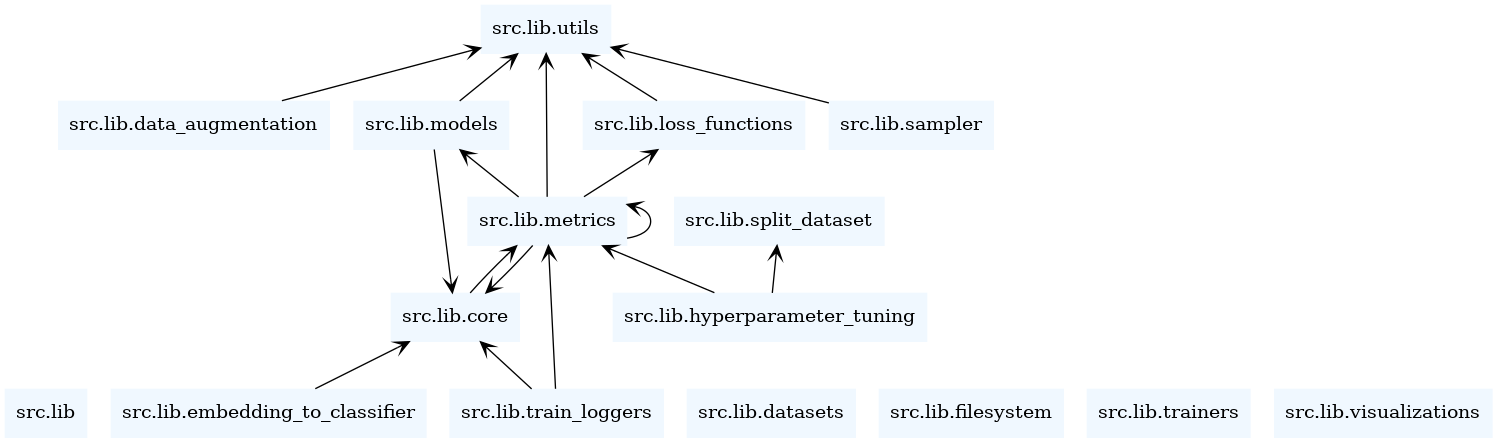
\includegraphics[width=0.8\textwidth]{informatica/diagrama_paquetes}
    \caption{Diagrama de paquetes de nuestra librería. Este diagrama ha sido creado usando la herramienta \lstinline{pyreverse}, que se ofrece como parte del programa \lstinline{pylint}.}
\end{figure}

Como deja claro el diagrama, hemos estructura el código de la librería en módulos muy interconectados entre ellos. Comentamos ahora el \textbf{propósito de los módulos más relevantes}:

\begin{itemize}
    \item \lstinline{src.lib.utils} contiene funciones auxiliares que se usan en distintas partes del código. Por ejemplo, comprobar si un tensor de \lstinline{pytorch} representa un vector o una matriz, realizar ciertos pre-cómputos para acelerar la ejecución de módulos, autentificarse en el servicio de logging \lstinline{wandb}, \ldots
    \item \lstinline{src.lib.loss_functions} contiene todo el código para computar las distintas funciones de pérdida que hemos introducido en \customref{ich:fundamentos_teoricos}.
    \item \lstinline{src.lib.sampler} contiene el código que implementa el \textit{P-K sampling}
    \item \lstinline{src.lib.metrics} implementa todas las métricas que hemos introducido en \customref{isec:metricas_teoria}
    \item \lstinline{src.lib.train_loggers} contiene la lógica para mostrar las métricas deseadas durante el ciclo de entrenamiento de forma cómoda, modular y extensible, como comentaremos en \customref{isec:loggin_metricas}
    \item \lstinline{src.lib.datasets} contiene la lógica para descargar, extraer, y cargar en una clase accesible para \lstinline{pytorch} los \textit{datasets} \textit{FG-Net} y \textit{CACD}

    \item \lstinline{src.lib.hyperparameter_tuning} contiene el código necesario para realizar \textit{hyperparameter tuning} usando \textit{K-Fold Cross Validation}
    \todo{Hacer aquí una referencia a esta técnica. Igual debería ir en la parte de teoría}

    \item \lstinline{src.lib.split_dataset} contiene el código para dividir un \textit{dataset} en dos porciones, usando dos técnicas distintas. La primera técnica consiste en separar el \textit{dataset} usando muestreo aleatorio. La segunda técnica consiste en realizar la separación usando muestreo aleatorio, pero asegurando que no existan individuos de una clase en ambos \textit{datasets} simultáneamente
    \item \lstinline{src.lib.data_augmentation} implementa el aumento de datos. Este aumento de datos es necesario porque, como hemos comentado en \customref{isubsubs:observaciones_conclusiones_pksampling}, para realizar \textit{P-K sampling} es obligatorio que todos los individuos tengan al menos $K$ imágenes asociadas. Realizamos el aumento de datos de forma clásica, añadiendo nuevos elementos a nuestro \textit{dataset}, y de forma \textit{lazy} o perezosa. En el aumento de datos \textit{lazy} no generamos nuevos elementos hasta que estos se solicitan en alguna parte del código. En \customref{isec:aumentado_datos} explicamos esto en detalle
\end{itemize}

Por la gran extensión de la base de código, mostrar el diagrama de clases completo no aporta apenas información. Pero mostraremos los diagramas de clase de ciertos módulos en \customref{isec:modulos_relevantes}, cuando esto aporte información relevante.

\section{Módulos relevantes} \label{isec:modulos_relevantes}

Por la extensión del proyecto no comentaremos cada módulo de código desarrollado. Sin embargo, en esta sección, estudiaremos algunos de los módulos más relevantes introducidos en \customref{isec:estructura_paquetes_modulos}.

\subsection{\textit{P-K sampling}}

En \customref{isubs:muestreo_datos_pk_sampling_teoria} hemos introducido nuevas técnicas para computar el \textit{Triplet Loss}. Una parte fundamental de estas técnicas consiste en realizar el \textit{P-K sampling}, que implementamos en el módulo \lstinline{src.lib.sampler}, en la clase \lstinline{CustomSampler}.

\begin{figure}[H]
    \centering
    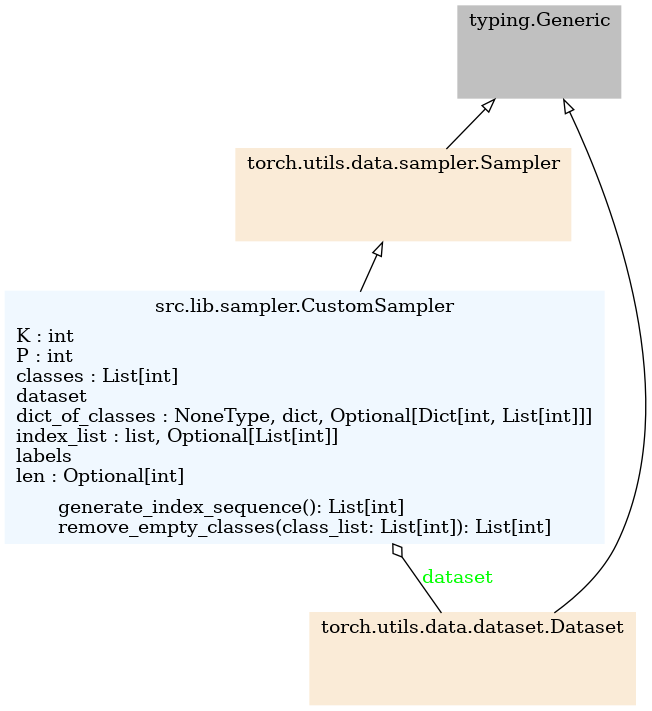
\includegraphics[width=0.6\textwidth]{informatica/pksampler_diagrama_clases}
    \caption{Diagrama de clases de \lstinline{CustomSampler} y sus clases colaboradoras. Este diagrama ha sido creado usando la herramienta \lstinline{pyreverse}, que se ofrece como parte del programa \lstinline{pylint}}
    \label{img:diagrama_clases_CustomSampler}
\end{figure}

En el diagrama de clases \customref{img:diagrama_clases_CustomSampler} podemos ver que:

\begin{itemize}
    \item \lstinline{CustomSampler} hereda de la clase \lstinline{Sampler} de \lstinline{torch} para introducir el comportamiento deseado a través de un \lstinline{Dataloader} \cite{informatica:pytorch_sampler}.
        \begin{itemize}
            \item Un \lstinline{DataLoader} especifica la forma en la que se realiza el \textit{batching} y otros detalles de implementación (por ejemplo, las políticas a seguir para cargar datos cuando trabajamos en paralelo). Uno de sus atributos es el \lstinline{sampler} usado. Escribiendo un \textit{sampler} propio será suficiente para obtener el comportamiento deseado
            \item Un \lstinline{Sampler} indica el orden en el que iteramos un \textit{dataset}. Debe implementar el método \lstinline{__len__()}, que muestra el número de datos que ofrecemos, y el método \lstinline{__iter__()}, que indica cómo se itera sobre los índices de los datos almacenados.
        \end{itemize}
\end{itemize}

En resumen, para realizar \textit{P-K sampling}, especificamos el orden el el que se itera el \textit{dataset} usando la clase \lstinline{CustomSampler}.

Fijados los valores de $P$ y $K$, debemos indicar que el \textit{batch size} sea $P \cdot K$. Esto es claro, pues de otra forma sería imposible generar \textit{batches} en los que haya $P$ individuos representados cada uno con $K$ imágenes.

El funcionamiento de \lstinline{CustomSampler} es el siguiente. Generamos una \textbf{lista de índices} vacía y una lista de imágenes candidatas, que al principio corresponderá al total del \textit{dataset}. Mientras al menos hayan $P$ individuos con al menos $K$ imágenes, realizamos el siguiente proceso:

\begin{enumerate}
    \item Elegimos aleatoriamente $P$ individuos asociados a la lista de imágenes candidatas
    \item Por cada individuo elegido, seleccionamos $K$ imágenes candidatas suyas aleatoriamente
    \item Añadimos los índices asociados a las $P \cdot K$ imágenes escogidas al final de la lista de índices y eliminamos dichas imágenes de la lista de candidatas
\end{enumerate}

Este proceso es realmente sencillo. Sin embargo, realizar optimizaciones para que consuma el menor tiempo posible complica su implementación. Principalmente hemos pre-computado algunos datos, que almacenamos como atributos, para acelerar este proceso:

\begin{itemize}
    \item \lstinline{self.dict_of_classes} es un diccionario en el que cada llave o \textit{key} es el identificador de un individuo (o su clase, en un entorno más amplio que el \textit{AIFR}) y el valor asociado a la llave es una lista de índices de imágenes de ese individuo. Con ello, una vez elegido un individuo al azar, es realmente rápido muestrear $K$ índices de imágenes asociadas
    \item \lstinline{self.classes} es una lista con los identificadores de individuos que tienen al menos $K$ imágenes, y por tanto, que son candidatos a ser elegidos en un ciclo del proceso anteriormente descrito
    \item Esto supone que, durante el proceso de generación de índices, debemos mantener en un estado válido estas estructuras, lo que añade algo de complejidad a la implementación, aunque supone una mejora en tiempos de ejecución considerable
\end{itemize}

\begin{observacion}

    Aunque los índices en cada \textit{P-K batch} estén ordenados por individuo, esto no supone un problema al considerar la definición de las funciones de pérdida que estamos usando (véase \customref{isubs:seleccion_de_triples})

\end{observacion}

\subsection{Aumentado de datos} \label{isec:aumentado_datos}

En \customref{isubsubs:observaciones_conclusiones_pksampling} hemos justificado la necesidad de llevar acabo aumentado de datos en ciertos \textit{datasets}, teniendo mucho cuidado de no saturar la memoria disponible. Por tanto, en el módulo \lstinline{src.lib.data_augmentation} proponemos dos soluciones, que mostramos en el siguiente diagrama de clases:

\begin{figure}[H]
    \centering
    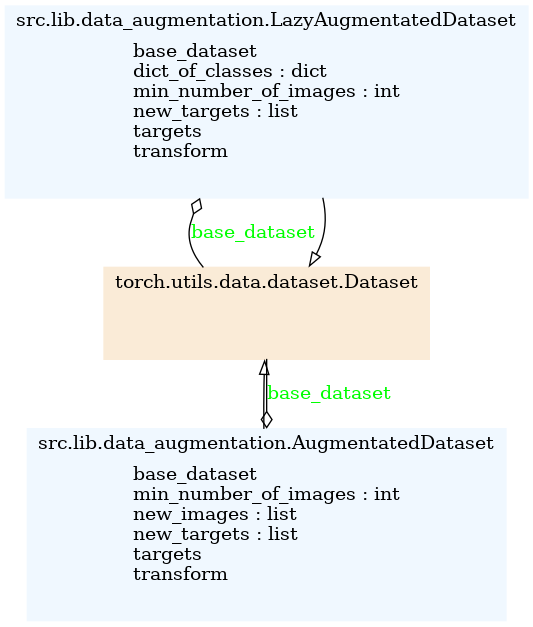
\includegraphics[width=0.6\textwidth]{informatica/diagramas_clases_aumentado_datos}
    \caption{Diagrama de clases de las dos soluciones propuestas para el aumentado de datos. Este diagrama ha sido creado usando la herramienta \lstinline{pyreverse}, que se ofrece como parte del programa \lstinline{pylint}}
    \label{img:diagrama_clases_aumentado_datos}
\end{figure}

En \customref{img:diagrama_clases_aumentado_datos} podemos ver que el aumentado de datos se realiza en dos clases que implementan la clase \lstinline{Dataset} de \lstinline{pytorch}. Gracias a esto, en nuestros \textit{pipelines} trabajamos igualmente con \textit{datasets} aumentados o sin aumentar, sin conocer este detalle. Además, podemos ver que ambas clases exponen la misma interfaz, por lo que podemos intercambiar estas soluciones. Podemos controlar cómo se generan nuevas imágenes gracias al atributo \lstinline{self.transform}.

Para trabajar con el aumentado de datos, indicamos el \textit{dataset} que queremos aumentar, \lstinline{self.base_dataset}, y el número de imágenes mínimo por individuo, \lstinline{self.min_number_of_images}. Dicho valor siempre lo establecemos al valor de $K$ que usemos en cada proceso de entrenamiento. Con ello, aseguramos que cada individuo puede participar en al menos un \textit{P-K batch}.

En \lstinline{AugmentedDataset}, localizamos los individuos con menos de \lstinline{self.min_number_of_images} imágenes asociadas. Generamos y almacenamos en memoria no permanente nuevas imágenes para estos individuos, en base a las imágenes que ya tenemos de los individuos. Almacenamos estas imágenes al final del \textit{dataset} (tienen los índices más altos). Pero esto no supone ningún problema gracias a estar usando \textit{P-K sampling}.

En \lstinline{LazyAugmentedDataset} localizamos los individuos con menos de \lstinline{self.min_number_of_images} imágenes asociadas. Generamos nuevos índices para estos individuos, que almacenamos como atributo, sin computar todavía las nuevas imágenes. Cuando queremos acceder a una imagen concreta identificada por un índice, comprobamos si este índice corresponde a una imagen original o una de las imágenes generadas por el aumento de datos. En el primer caso, devolvemos la imagen que ya tenemos almacenada en el conjunto de datos \lstinline{self.base_dataset}. En el segundo caso, generamos la imagen en ese preciso instante y la devolvemos. En ningún momento almacenamos la nueva imagen para su uso posterior.

El aumento de datos puede llegar a generar muchísimas imágenes nuevas si la distribución de número de imágenes por individuo es mala (como ocurre en \textit{LFW}). Por tanto, el proceso de almacenar las imágenes en memoria que hacemos en \lstinline{AugmentedDataset} puede provocar que saturemos la memoria disponible y que el proceso se detenga. Esto motiva el diseño de \lstinline{LazyAugmentedDataset}, que no almacena imágenes en memoria para su posterior uso.

No almacenar las nuevas imágenes en memoria supone el siguiente compromiso:

\begin{itemize}
    \item Si accedemos dos veces al mismo índice no obtenemos la misma imagen
    \item No se produce un aumento en el consumo de memoria, porque no estamos almacenando ninguna imagen nueva
    \item El proceso de crear un \textit{dataset} aumentado es más rápido. Pero el acceso a nuevos datos es más lento. En la variante \textit{lazy} tenemos que esperar a que se genere la nueva imagen. Mientras que en la variante normal, ese proceso ya se ha realizado previamente y el acceso es inmediato
\end{itemize}

Para realizar el aumento de datos estamos utilizando:

\begin{itemize}
    \item Un cortado aleatorio de la imagen, usando \lstinline{torchvision.transforms.RandomResizedCrop}. Dicho método toma una porción aleatoria de la imagen, y cambia su tamaño al especificado en la función. El tamaño de las imágenes producidas es igual al tamaño de las imágenes originales
    \item Una rotación aleatoria, usando \lstinline{torchvision.transforms.RandomRotation}. Rotamos entre 0º y 20º
    \item Un cambio de contraste aleatorio, usando \lstinline{torchvision.transforms.RandomAutocontrast}
\end{itemize}

\subsection{Implementaciones propias de \textit{Datasets}} \label{isec:datasets_customs}

Como ya hemos comentado en \customref{isec:base_datos_usada}, las bases de datos \textit{FG-Net} y \textit{CACD} no se ofrecen como parte de ninguna librería asociada a \lstinline{Pytorch}. Por tanto, tendremos que implementar la descarga, extracción y carga en objetos compatibles con \lstinline{Pytorch}. Estas tareas se realizan en el módulo \lstinline{src/lib/datasets}.

Este módulo contiene, además de las dos clases que más adelante estudiamos, las funciones \lstinline{download_fg_dataset} y \lstinline{download_cacd_dataset}, que descargan y extraen los dos \textit{datsets}.

\begin{figure}[H]
    \centering
    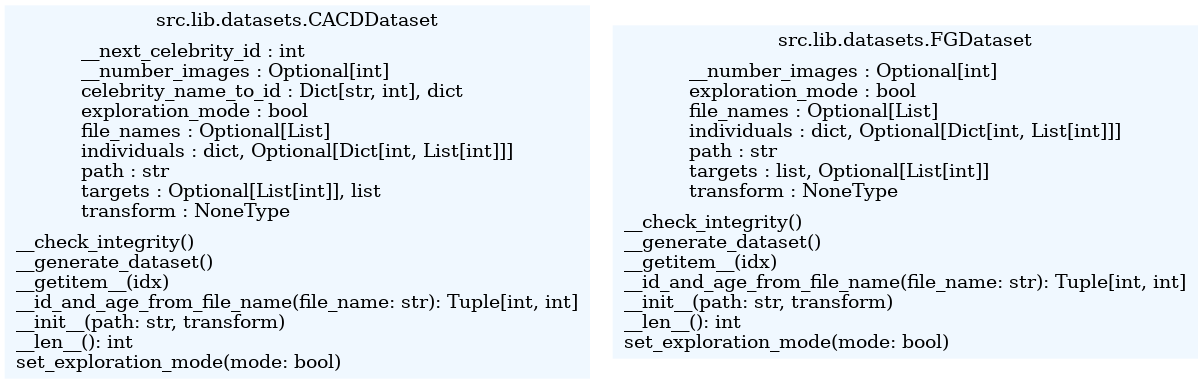
\includegraphics[width=0.6\textwidth]{informatica/diagrama_clases_carga_datos}
    \caption{Diagrama de clases de las implementaciones para los \textit{datasets} \textit{FG-Net} y \textit{CACD}. Este diagrama ha sido creado usando la herramienta \lstinline{pyreverse}, que se ofrece como parte del programa \lstinline{pylint}}
    \label{img:diagrama_clases_datasets}
\end{figure}

En \customref{img:diagrama_clases_datasets} podemos ver el diagrama de clases de las dos implementaciones realizadas. Para inicializar estas clases, solo tenemos que especificar la localización del directorio donde se almacenan los datos.

Para poder trabajar correctamente con \lstinline{Pytorch}, debemos especificar el tamaño del \textit{dataset} con el método \lstinline{__len__()} e implementar el acceso a cada elemento del \textit{dataset} con el método \lstinline{__getitem__()}.

A la hora de cargar los datos al \textit{dataset}, realizamos el siguiente proceso:

\begin{itemize}
    \item Tomamos los nombres de todas las imágenes almacenadas en el \textit{dataset}, que guardamos en el atributo \lstinline{self.file_names}
    \item A partir de los nombres de las imágenes, extraemos el identificador y edad asociados a cada imagen. Para ello usamos el método \lstinline{__id_and_age_from_filename(filename: str)}
    \item Almacenamos adecuadamente toda esta información para poder devolver dicha información en \lstinline{__getitem__}
\end{itemize}

El método \lstinline{check_integrity()} comprueba el tamaño del \textit{dataset} para asegurarnos de que no ha habido corrupción de datos en la descarga. El método \lstinline{set_exploration_mode()} permite activar el modo exploración. En dicho modo, \lstinline{__getitem__()} devuelve la imagen con una serie de metadatos asociados almacenados en un diccionario (edad e identidad). En el modo de funcionamiento normal, \lstinline{__getitem__()} devuelve un par con la imagen y la etiqueta de dicha imagen.

\subsection{Normalización}

En \customref{isec:triplet_loss} hemos comentado el problema que puede suponer que la red aprenda a colapsar cualquier entrada al vector $\vec{0}$. Aunque añadimos un margen $\alpha$ para evitar este comportamiento, en \customref{isec:margenes_suaves} introducimos una variante en la que podría llegar a aprenderse este mal comportamiento. Por tanto, otra técnica a explorar es la de normalizar las salidas de la red, forzando a que tengan norma unitaria. Esta técnica se usa en \cite{informatica:facenet}. La normalización consiste en realizar la siguiente sustitución:

\begin{equation} \label{ieq:normalizacion}
    \hat{x} := \frac{f_{\theta}(x)}{||f_{\theta}(x)||_2}
\end{equation}

Además del interés que pueda tener estudiar el comportamiento de los modelos al introducir la normalización, esta técnica introduce el siguiente punto a tener en cuenta. Durante los entrenamientos hemos tenido muchos problemas de inestabilidad. Esto es, en la mayoría de ocasiones, el entrenamiento se saturaba tras pocas iteraciones. Es claro que si nuestra red aprende a colapsar todas las entradas a $\vec{0}$, la ecuación \eqref{ieq:normalizacion} falla, con lo que el entrenamiento se detiene. Sin embargo, a raíz de la experimentación, vemos que la normalización ayuda enormemente a que dicho comportamiento no se aprenda. Y con ello, es mucho más fácil conseguir entrenamientos estables. El siguiente diagrama muestra un ejemplo de entrenamiento inestable:

\begin{figure}[H]
    \centering
    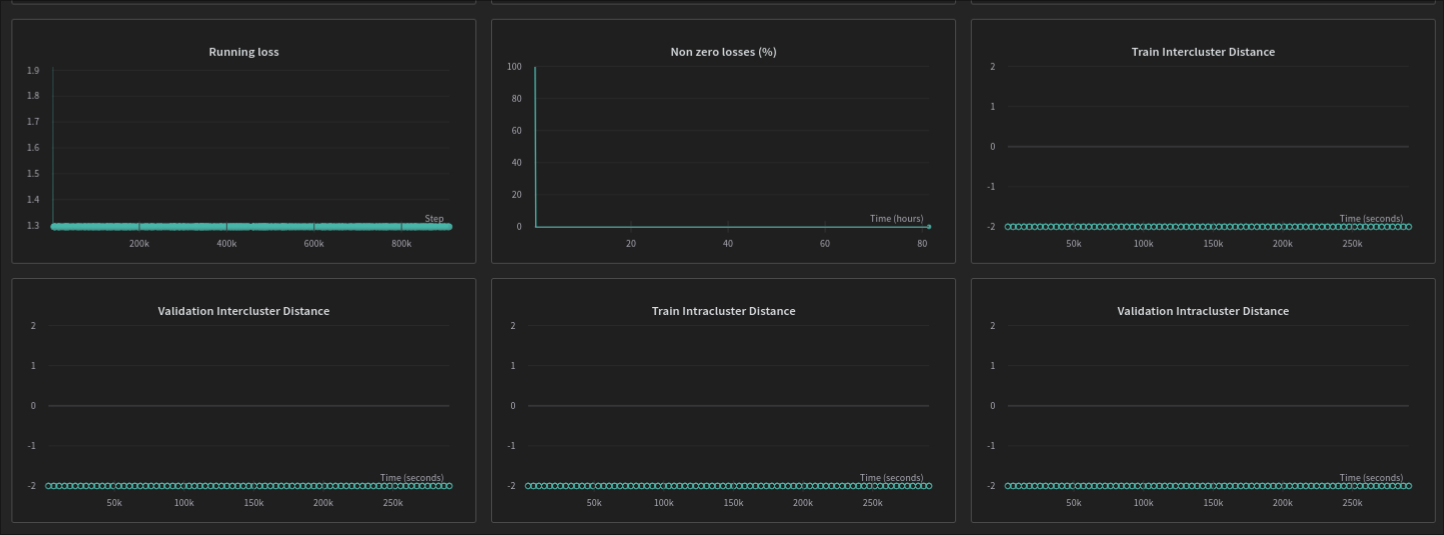
\includegraphics[width=0.8\textwidth]{informatica/ejemplo_colapso_entrenamiento}
    \caption{Histórico de \textit{WANDB} que muestra un entrenamiento inestable que acaba por fallar. En las gráficas, los círculos indican entradas con el valor \lstinline{NaN}}
\end{figure}

Nuestro objetivo es introducir esta normalización en nuestros modelos de aprendizaje automático, de forma modular y sencilla. En el módulo \lstinline{src.lib.models}, donde describimos las arquitecturas empleadas a lo largo de toda la experimentación, definimos la clase \lstinline{NormalizedNet}. Dicha clase implementa el patrón de diseño \textit{Composite}, del que ya hemos hablado en \customref{isec:loggin_metricas}.

Esta clase toma una red neuronal como parámetro. Las redes neuronales de \lstinline{pytorch} deben implementar el método \lstinline{forward}, que indica cómo la red computa las salidas a partir de las entradas dadas. Nuestra clase \lstinline{NormalizedNet} implementa este método basándose en el mismo método de la clase base. Usamos el método \lstinline{forward} de la clase base y almacenamos la salida, que normalizamos y devolvemos.

El uso de este patrón supone que no estamos cambiando la interfaz de un modelo si lo normalizamos, lo que permite que podamos decidir si queremos trabajar o no con normalización sin que el resto del código tenga que saber esto. Por ejemplo:

\begin{lstlisting}[caption={Ejemplo de uso del patrón \textit{composite} para decidir si usamos o no normalización. El resto del código no tiene por qué saber este detalle de implementación, porque no cambiamos la interfaz de la clase}, captionpos=b]
net = LFWResNet18(embedding_dimension = 5)
net = NormalizedNet(net)
\end{lstlisting}

\subsection{\textit{Hyperparameter Tuning}} \label{isec:hp_tuning}

\subsection{Adaptadores para realizar \textit{retrieval}}

\subsection{Separación de datos teniendo en cuenta obtener clases disjuntas}
\todo{Merece la pena comentar esto?}

\subsection{Logging de métricas} \label{isec:loggin_metricas}

\begin{figure}[H]
    \centering
    % 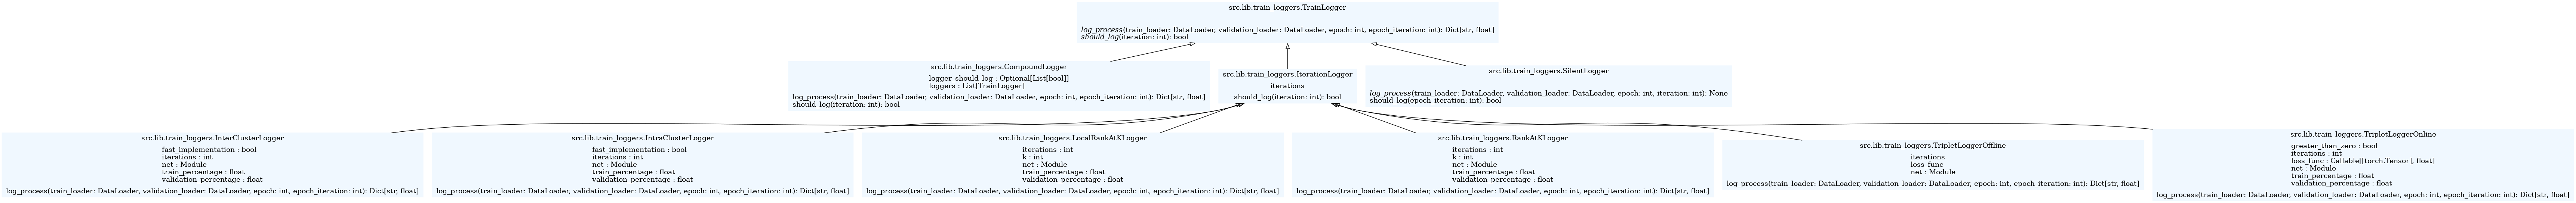
\includegraphics[width=0.8\textwidth]{informatica/diagrama_loggers}
    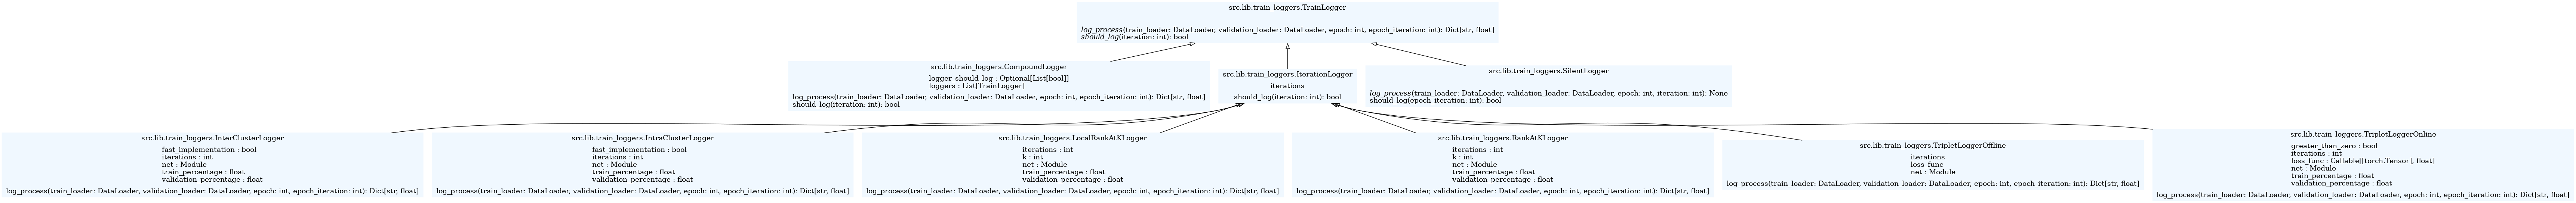
\includegraphics[width=1.25\textwidth,height=\textheight,keepaspectratio]{informatica/diagrama_loggers}
    \caption{Diagrama de clases del módulo \lstinline{src.lib.train_loggers}. Este diagrama ha sido creado usando la herramienta \lstinline{pyreverse}, que se ofrece como parte del programa \lstinline{pylint}}
    \label{img:diagrama_clases_loggers}
\end{figure}

El módulo \lstinline{src.lib.train_loggers} se encarga de introducir el cálculo y visualización de métricas en el proceso de entrenamiento de forma cómoda, modular y extensible. Nuestro objetivo es definir el proceso de \textit{logging} de forma externa al bucle de entrenamiento. De esta forma, podremos cambiar las métricas observadas sin tener que modificar el código que implementa el bucle de entrenamiento.

En \customref{img:diagrama_clases_loggers} podemos ver la siguiente estructura:

\begin{itemize}
    \item La clase abstracta \lstinline{Trainlogger} define la interfaz que queremos que todos los \textit{loggers} implementen. Dicha interfaz se compone de dos métodos:
        \begin{itemize}
            \item \lstinline{log_process} que muestra los valores de ciertas métricas tomando como entradas los datos de entrenamiento, los datos de validación, la época en la que nos encontramos en el proceso de entrenamiento y la iteración dentro de dicha épica
            \item \lstinline{should_log} que decide si debemos mostrar o no las métricas para una iteración global del proceso de entrenamiento
        \end{itemize}
    \item Gracias a esta interfaz, el bucle de entrenamiento puede mostrar métricas solo cuando \lstinline{should_log} lo indique, pasando todos los datos necesarios a \lstinline{log_process}
    \item La clase \lstinline{SilentLogger} ofrece una implementación trivial de la interfaz. \lstinline{should_log} siempre devuelve falso y \lstinline{log_process} no realiza ninguna acción
    \item El resto de clases tienen la misma lógica para decidir cuándo mostrar las métricas. Por tanto, la clase abstracta \lstinline{IterationLogger} implementa dicha lógica compartida, dejando todavía como método abstracto a \lstinline{log_process}
    \item Los \textit{loggers} que vemos en la parte baja del diagrama son \textit{loggers} concretos que implementan cada uno \lstinline{log_process} con el cálculo y visualización de métricas concretas
    \item La clase \lstinline{CompoundLogger} implementa el \textbf{patrón de diseño \textit{composite}}
\end{itemize}

Como acabamos de comentar, la clase \lstinline{CompoundLogger} implementa el patrón de diseño \textit{composite} \cite{informatica:design_patterns}. En dicho patrón buscamos definir la lógica de ciertos componentes en función del agregado de otros componentes. En nuestro caso, buscamos definir un objeto que implemente la interfaz \lstinline{TrainLogger} combinando varios \textit{loggers} en uno solo. Para ello, guardamos una lista de objetos de tipo \lstinline{TrainLogger}. La función \lstinline{should_log} consulta a todos los objetos guardados si quieren mostrar métricas, haciendo uso de la misma función \lstinline{should_log}. En cuyo caso, se llama a los correspondientes métodos \lstinline{log_process}. Gracias a esto, en un \textit{script} de \lstinline{Python} podemos configurar nuestro \textit{logging} con el siguiente código:

\begin{lstlisting}[language=python, caption=Ejemplo de configuración del \textit{logging} de un entrenamiento con nuestro sistema propio. Se ve claramente la ventaja de usar un patrón \textit{composite} a la hora de configurar qué \textit{loggers} queremos usar, captionpos=b]

# Define the loggers we want to use
triplet_loss_logger = TripletLoggerOnline(... params ... )
cluster_sizes_logger = IntraClusterLogger(... params ... )
intercluster_metrics_logger = InterClusterLogger( ... params ... )
rank_at_one_logger = RankAtKLogger( ... params ... )
rank_at_k_logger = RankAtKLogger( ... params ... )
local_rank_at_one_logger = LocalRankAtKLogger( ... params ... )
local_rank_at_k_logger = LocalRankAtKLogger( ... params ... )

# Combine them in a single logger
logger = CompoundLogger([
    triplet_loss_logger,
    cluster_sizes_logger,
    intercluster_metrics_logger,
    rank_at_one_logger,
    rank_at_k_logger,
    local_rank_at_one_logger,
    local_rank_at_k_logger,
])
\end{lstlisting}

Hemos usado \textbf{dos técnicas para mostrar las métricas calculadas}. La primera y más sencilla ha sido \textbf{imprimir por pantalla} los valores obtenidos. Esta técnica no es suficiente porque no podemos guardar de forma estructurada los históricos de entrenamientos, ni facilita estudiar de forma visual el comportamiento del entrenamiento. Por tanto, hemos usado como segunda técnica el servicio \textbf{\textit{Weights and Biases} o \textit{WANDB}} \cite{informatica:wandb_web}. Este servicio permite registrar métricas de forma muy sencilla, relegando en dicho servicio:

\begin{itemize}
    \item El control de históricos de entrenamiento
    \item La visualización de los procesos de entrenamiento
    \item El registro de parámetros globales usados en cada entrenamiento
\end{itemize}

Para registrar todos los parámetros globales, creamos un diccionario de \lstinline{Python} en el que definimos dichos parámetros. Este diccionario, al que llamamos \lstinline{GLOBALS}, se registra directamente en la plataforma \textit{WANDB}. Los parámetros globales definen hiperparámetros del proceso de entrenamiento (por ejemplo, los valores de $\{P, K\}$), directorios en los que guardamos archivos, qué entorno de ejecución estamos usando, si queremos saltar ciertas secciones del \textit{pipeline}, \ldots

A continuación mostramos un ejemplo de uso de esta plataforma:

\begin{figure}[H]
    \centering
    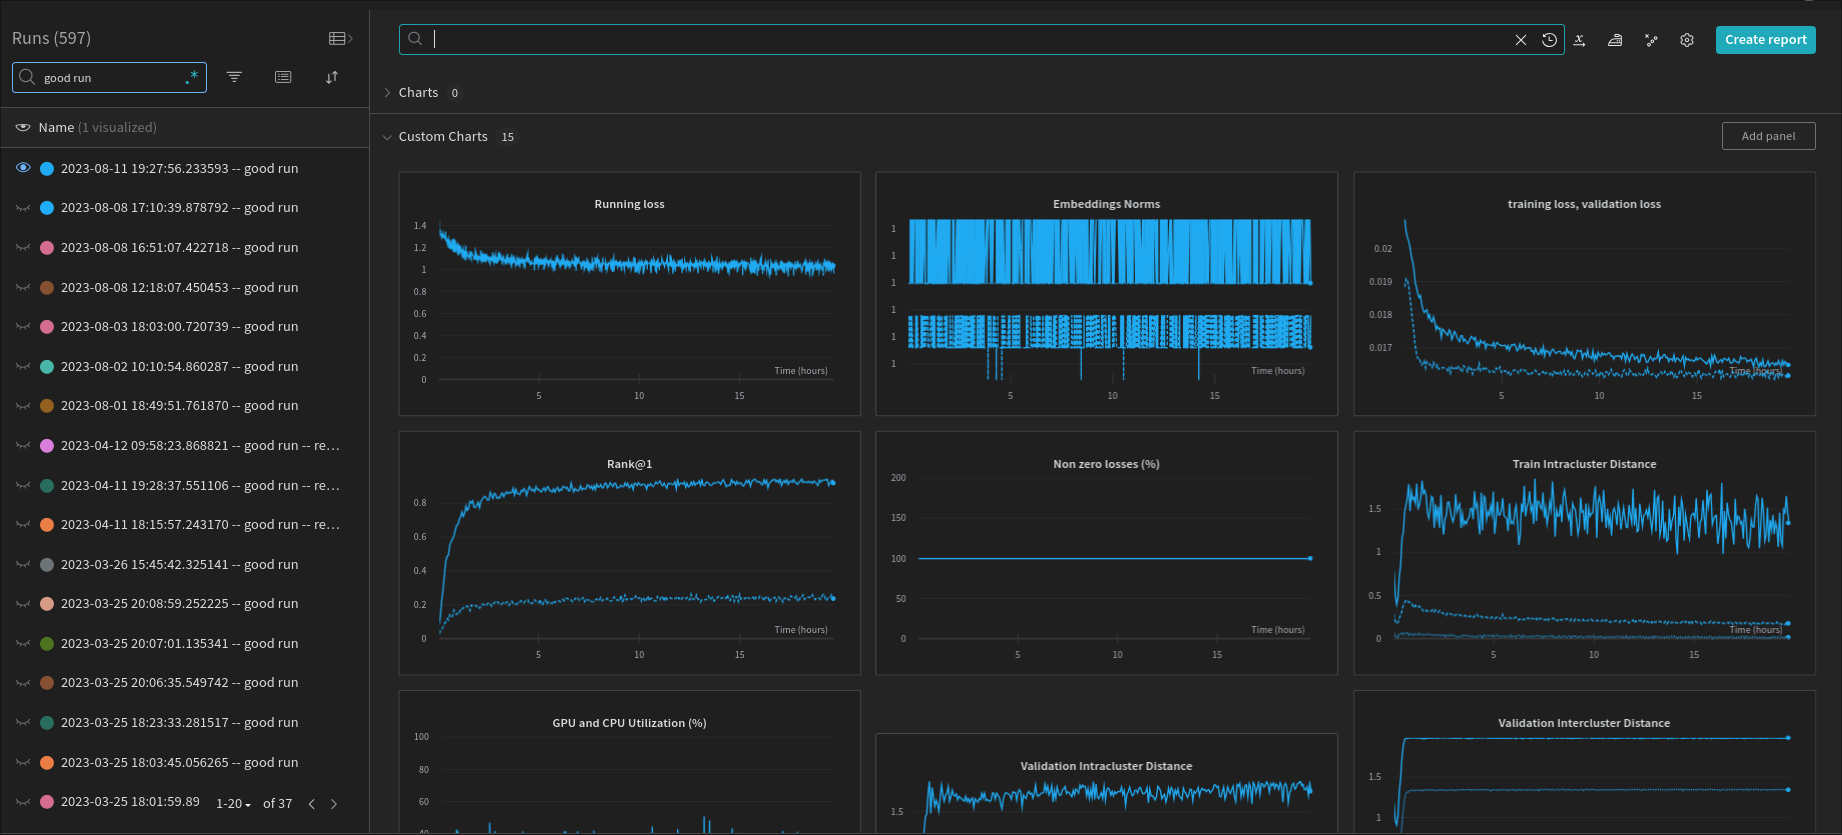
\includegraphics[width=0.8\textwidth]{informatica/wandb_example}
    \caption{Ejemplo de uso de \textit{WANDB}. A la izquierda, podemos ver una lista filtrada para mostrar solo los históricos que producen resultados satisfactorios. A la derecha, podemos ver algunas métricas recogidas por nuestro sistema de \textit{logging}}
\end{figure}

\section{Optimización del código} \label{isec:optimizacion_codigo}

\section{Pipeline} \label{isec:pipeline}

\section{\textit{Suite} de \textit{tests}} \label{isec:test_suite}

Disponemos de dos conjuntos o \textit{suites} de \textit{tests}: unitarios y de integración.

Los \textbf{\textit{tests} unitarios} buscan principalmente validar la corrección de los módulos de código desarrollados en la librería. Para ello, usamos algunas técnicas comunes de \textit{testeo}:

\begin{itemize}
    \item Validación de casos concretos: controlamos los datos de entrada de una funcionalidad, y comprobamos la salida con el resultado esperado. Esto es factible cuando las funciones a validar son deterministas y fáciles de calcular manualmente. Como puede ser el caso de las funciones de pérdida, validadas en \lstinline{src/test/loss_functions.py} usando principalmente este enfoque
    \item Validación de propiedades \cite{informatica:property_based_testing}: dados unos datos de entrada, comprobamos que ciertas propiedades de la funcionalidad a validar se cumplen. Esta técnica es realmente útil cuando usamos funciones no deterministas, o cuando no es viable computar manualmente la salida esperada. Como puede ser el caso del aumentado de datos (véase \customref{isec:aumentado_datos}), de naturaleza claramente aleatoria. Comprobamos propiedades como:

    \begin{itemize}
        \item Que el tamaño del \textit{dataset} no aumenta si todos los individuos tienen al menos $K$ imágenes asociadas
        \item Que tras el aumento de datos todos los individuos tienen al menos $K$ imágenes asociadas
        \item Que el tamaño del \textit{dataset} aumenta o se mantiene, nunca disminuye
    \end{itemize}

\end{itemize}

También usamos \textit{tests} unitarios cada vez que encontramos un error en nuestra base de código, siguiendo el siguiente proceso:

\begin{itemize}
    \item Aislamos el error en una serie de \textit{tests} que comprueban la propiedad que no se está cumpliendo
    \item Tratamos de localizar y arreglar la fuente del error
    \item Comprobamos que, tras arreglar el problema, los \textit{tests} introducidos ahora sí que se ejecutan correctamente
\end{itemize}

Esto permite encontrar y solucionar los problemas más rápidamente, y además documentar errores previamente encontrados y propiedades que son importantes verificar en otros escenarios.

Los \textbf{\textit{tests} de integración} buscan evitar el siguiente problema. Como hemos comentado en \customref{isec:planificacion}, hemos realizado un trabajo iterativo, partiendo de bases de datos más sencillas hacia bases de datos más grandes y complejas. En dicho trabajo iterativo puede ocurrir que, cambiando o añadiendo código a la librería, rompamos \textit{pipelines} en bases de datos previas. Los \textit{tests} de integración buscan verificar que \textit{pipelines} en bases de datos previas sigan funcionando.

Para esto, cada \textit{test} de integración ejecuta el \textit{pipeline} de una base de datos cuando abandonamos esta para pasar a la siguiente. Usamos valores de los parámetros para adecuar la tarea: usamos un subconjunto muy reducido de la base de datos, hacemos \textit{logging} de forma mucho menos frecuente, los valores de $\{P, K\}$ son mucho más bajos, la red neuronal es muy ligera, ...

Por el esfuerzo computacional que suponen, los \textit{tests} de integración únicamente se ejecutan a la hora de validar una \textit{pull request}.

Y como ya hemos comentado en \customref{isec:github_buenas_practicas}, estamos usando \textit{Github Actions} para lanzar las dos \textit{suites} de \textit{tests}, aunque usando la herramienta \lstinline{just} (véase \customref{isec:estructura_carpetas}) se pueden lanzar en local.
